\documentclass[UTF8]{ctexart}
\usepackage{bookmark}
\usepackage{geometry}
\usepackage{hyperref}
\geometry{a4paper,scale=0.8}
\usepackage{ctex}
\usepackage[style=caspervector,backend=biber,utf8]{biblatex}
\usepackage{booktabs}
\usepackage{array}
\usepackage{fancyhdr}
\pagestyle{fancy}
\fancyhf{}
\renewcommand\footrulewidth{1pt}
\lhead{\textit{王铠泽}}
\rhead{\textit{PB18020766}}
\chead{\href{mailto:volar@mail.ustc.edu.cn}{\textit{volar@mail.ustc.edu.cn}}}
\rfoot{\href{http://en.ustc.edu.cn/}{\textit{中国科学技术大学}}}
\lfoot{\today}
\usepackage{graphicx}
\usepackage{float}
\usepackage{subfigure}
\fancyfoot[C]{\thepage}


\begin{document}

	\centering\textbf{\LARGE{计算物理A第十一次作业}}
	
	\pagenumbering{arabic}
	\textit{王铠泽\qquad PB18020766}
	
		
	\section{作业题目}
	
	\begin{itemize}
		\item 数值研究$  d(d=1, 2, 3) $维空间中随机行走返回原点的几率 $ P_d $,讨论它随
		步数 $ N $ 的变化关系 $ P_d(N) $,能否定义相关的指数值?
		
	\end{itemize}

	\section{实现方法和原理}
	
	\begin{itemize}
		\item $d$ 维随机游走的实现
		
		本次实验采用离散化模型,即一维链,二维正方形网格,三维正方体网络来摸拟$d$维的随机游走。具体到算法上,采用$16807$产生器每一次产生一个$[0,1]$之间的随机数$\xi$,若$\xi>0.5$,则朝正方向前进一步;若$\xi<0.5$,则朝负方向前进一步。使用计数器$cnt$来计数在第$N$步返回原点的次数,除以总系统数量$M$,就可以得到第$N$步返回原点的概率$p(N)$。
		
		\item $d$ 随机游走理论和常返性
		
		对于网格模型,显然只有在偶数步$N$时才能返回原点(奇数步必然在正负两个方向中有一个是多出一部分步长的)。
		
		\subitem 一维情形
		$$p(N)=\frac{N!}{(\frac{N}{2}!)^2}\left( \frac{1}{2}\right) ^{N}$$
		
		
		\subitem 二维情形
		$$p(N)=\sum_{k=0}^{\frac{N}{2}}\frac{N!}{[k!\cdot(\frac{N}{2}-k)!]^2}\left( \frac{1}{4}\right)^{N}$$
		
		\subitem 三维情形
		$$p(N)=\sum_{k=0}^{\frac{N}{2}}\sum_{j=0}^{\frac{N}{2}-k}\frac{N!}{[k!\cdot j!\cdot(\frac{N}{2}-k-j)!]^2}\left( \frac{1}{6}\right)^{N}$$
		
		当步数$N$足够大的时候,做$Stirling$近似展开得到$d$维随机游走标度律为[1]:
		
		$$p^{2N}(0,0)=C_dN^{-\frac{d}{2}}$$
		
		对三维情况简单的证明如下:
		
		每一步要决定是走南北、东西、上下哪一个方向,那么总共有$C^{N}_{2N}$种组合方式取安排总共$N$步走南东上,$N$步走北西下。那么必然也有$i$步走南/北,$j$步走东/西,$N-i-j$步走上/下。从而:
		
		$$p^{2N}(0,0)=\frac{1}{6^{2N}}C^{N}_{2N}\left( \sum_{i+j\leq N}\frac{N!}{i!j!(N-i-j)!}\right) ^2$$
		
		可以验证,在$x+y+z=N$,$N$充分大,当$x=y=z=\frac{N}{3}$时,$x!y!z!$取得最小值。
		
		所以
		
		$$p^{2N}(0,0)\leq\frac{1}{6^{2N}}C^{N}_{2N}\frac{N!}{\frac{N}{3}!^2}\left( \sum_{i+j\leq N}\frac{N!}{i!j!(N-i-j)!}\right)=\frac{1}{6^{2N}}C^{N}_{2N}\frac{N!}{{(\frac{N}{3}!)}^23^{N}}\sim C_3N^{-3/2}$$
			
		
		
		常返性可以通过$\sum_{N=0}^{\infty}p^{2N}(0,0)$的收敛性来判断,这是由过程的马尔可夫性决定的。一,二维上该级数发散,所以是常返的。三维以上发散,不再常返[1]。
		\end{itemize}
		
	\section{程式说明}
	
	
	\begin{itemize}
		\item random\_walk.c
		
		该程式输出在 $d=1,2,3$维情况下的$P_1(N),P_2(N),P_3(N)$。
		
		\item ideal.c
		
		该程式输出在 $d=1,2,3$维情况下的理论$P_1(N),P_2(N),P_3(N)$。
		
		\item rdm.h
			
		这是一个包含了使用16807产生器生成指定长度的$[0,1]$上均匀分布随机数函数的头文件。
		
		\subitem void rdm(int N,double *x,int method)
		
		该函数将输入的指针$x$对应的长度为$N$的数组用$[0,1]$上的随机数填满。method是关于初始种子的选择。method=0:默认种子;method=1,时间种子。程式中故意采用$sleep$函数就是为了得到不同的时间种子。
		
		\item time\_seed.txt
		
		16807产生器抽样时对应的时间种子数据(每次1个种子)。调用多少次16807生成器就生成多少个数据记录。每一个分布对应的种子已经手动加上对应的实验了。种子产生公式如下:
		
%		
		\begin{figure}[H]
			\centering  %图片全局居中
			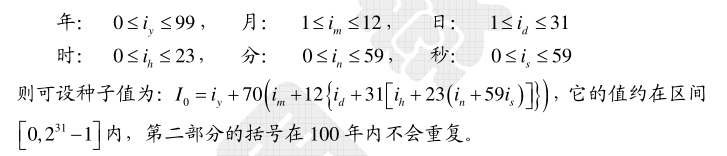
\includegraphics[width=4in]{1.png}
		\end{figure}
%		
\textbf{		Tip:程序中多处使用了$sleep$函数是为了换时间种子,因而可能运行时间较久一点。}
	
		\item 1/2/3d\_random\_walk.txt
		
		记录了$p(N)$的txt文件
		
		\item 1/2/3d\_ideal.txt
		
		记录了理论上从$N=1\sim200$的$p(N)$数值,后续作图和实验值作比较。
		
		
	\end{itemize}
	
	\section{计算结果}

	
			\begin{flushleft}
				选择总步数为$N=1000$,系综包含的系统数为$M=200000$个。以网格模型摸拟随机游走,得到的结果如下:
			\end{flushleft}


	
	\subsection{不同维度下$p(N)$和理想结果的对比}
%	
			\begin{figure}[H]
					\centering  %图片全局居中
					\subfigure[$p_{1d}(N)$]{
						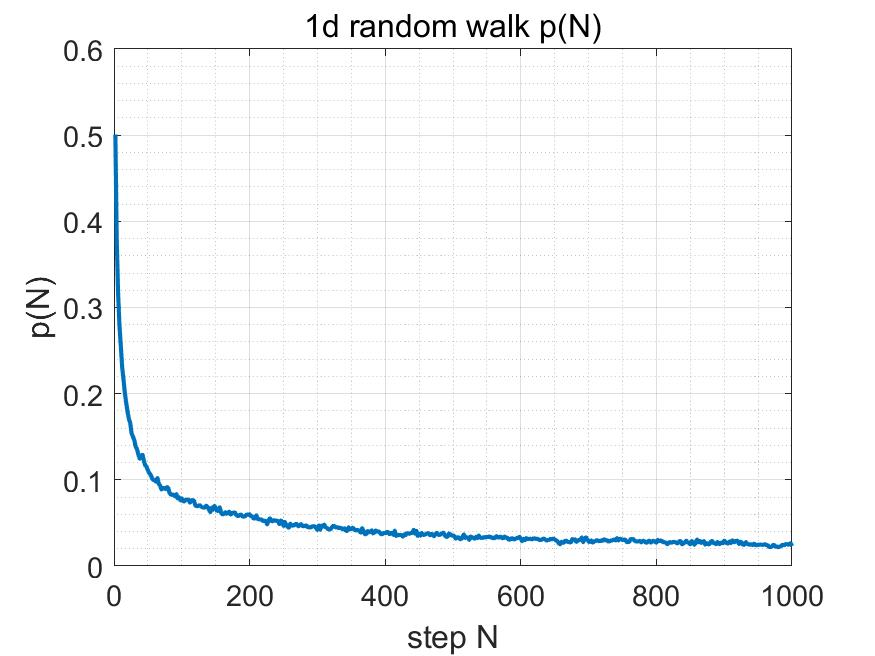
\includegraphics[width=0.6\textwidth]{../result_1/1d.jpg}}
				\subfigure[与理想值的比较(圆圈为理想值)]{
					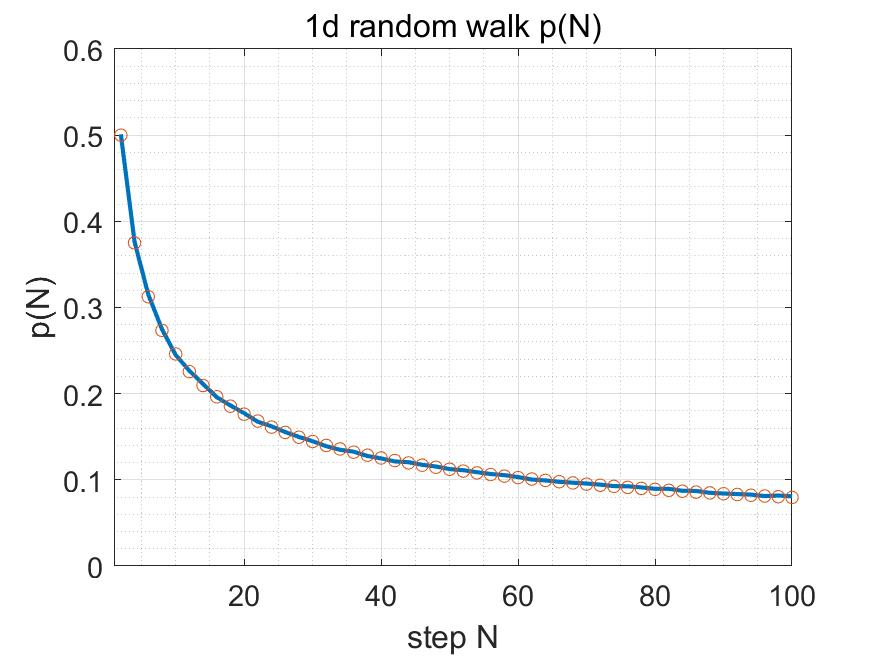
\includegraphics[width=0.6\textwidth]{../result_1/1d_2.jpg}}
					\caption{一维情形}
				\end{figure}
		\clearpage	
		\begin{figure}[htbp]
		\centering  %图片全局居中
		\subfigure[$p_{2d}(N)$]{
			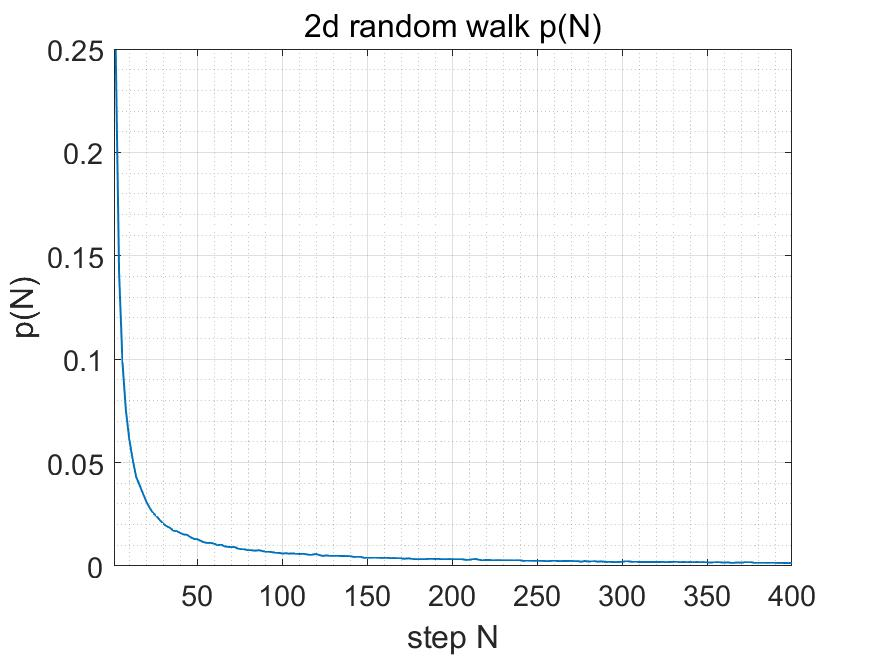
\includegraphics[width=0.6\textwidth]{../result_1/2d.jpg}}
		\subfigure[与理想值的比较(圆圈为理想值)]{
			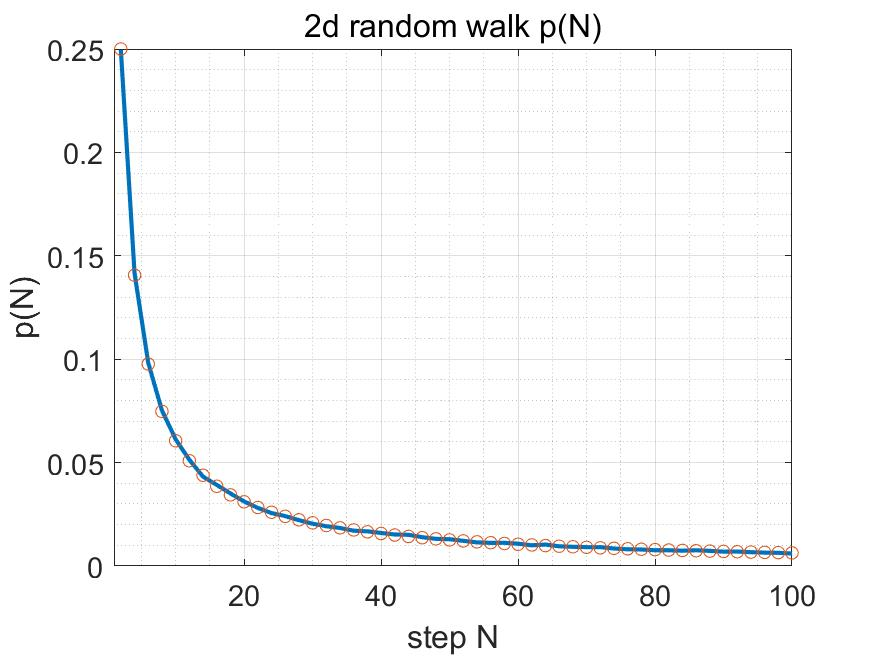
\includegraphics[width=0.6\textwidth]{../result_1/2d_2.jpg}}
		\caption{二维情形}
	\end{figure}
		\clearpage
			\begin{figure}[htbp]
			\centering  %图片全局居中
			\subfigure[$p_{3d}(N)$]{
				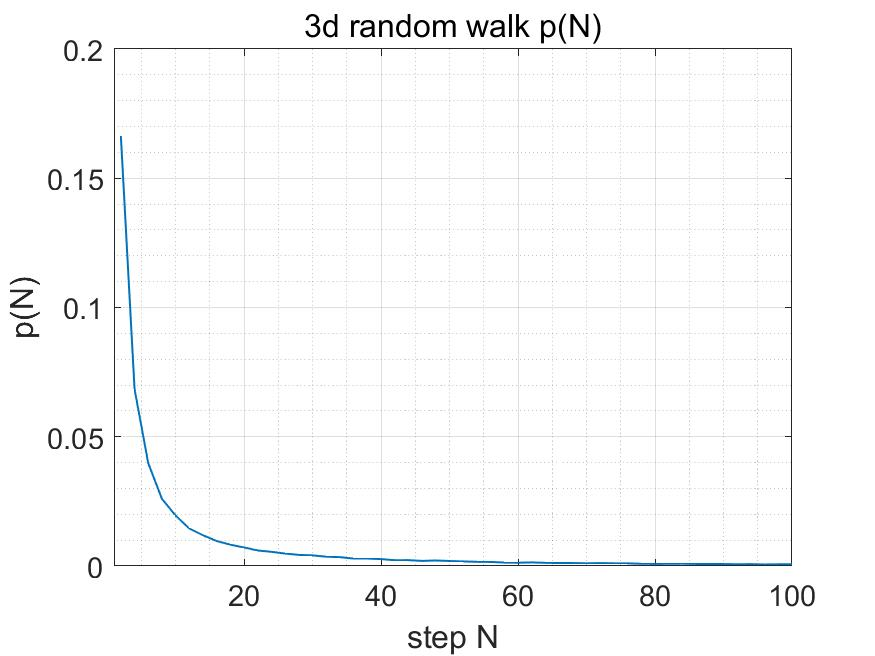
\includegraphics[width=0.6\textwidth]{../result_1/3d.jpg}}
			\subfigure[与理想值的比较(圆圈为理想值)]{
				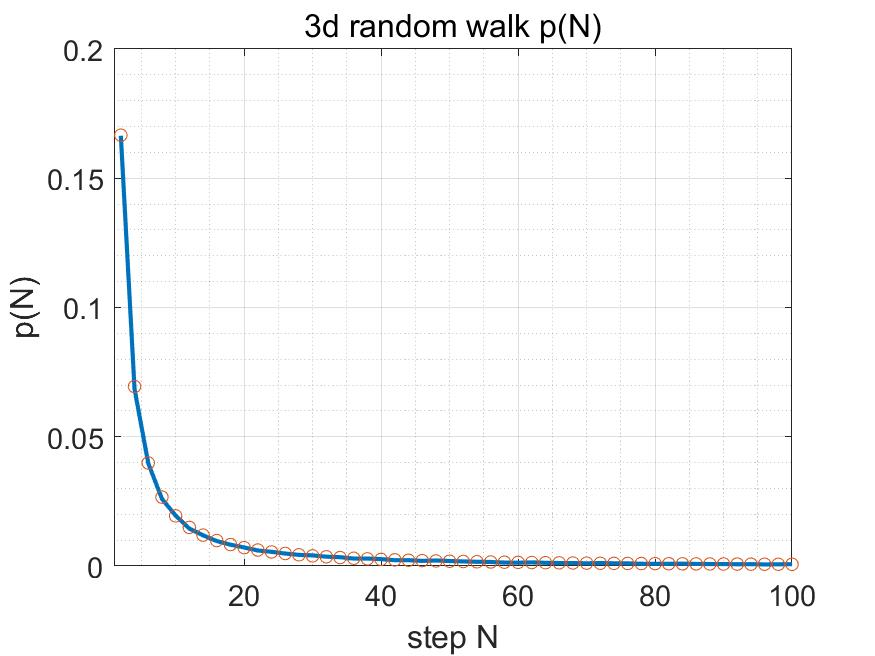
\includegraphics[width=0.6\textwidth]{../result_1/3d_2.jpg}}
			\caption{三维情形}
		\end{figure}
	
	
\begin{flushleft}
		从上面的计算结果可以看出,我们的计算模拟和理论计算值非常吻合。除了少许的涨落,得到的曲线基本满足前面的理论推导。
\end{flushleft}
	
	
	
	\subsection{标度律指数的计算}

	对$d=1,2,3$维分别做出双对数图,计算指数标度律如下
%	
	\begin{figure}[H]
		\centering  %图片全局居中
		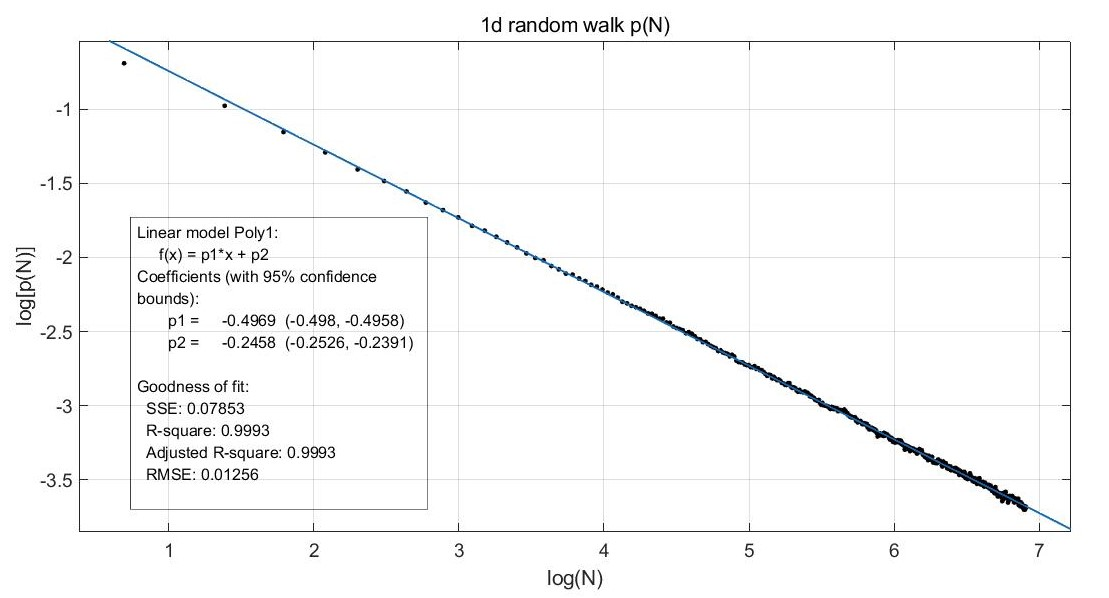
\includegraphics[width=6in]{../result_1/curve_1d.jpg}
		\caption{1d随机游走}
	\end{figure}
%	
	\begin{flushleft}
		从拟合结果来看,一维的指数大约为$\nu=\textbf{-0.4969}$。这和理论近似的$\textbf{-0.5}$非常接近,且随着$N$的增大,吻合程度增大,这也符合对大$N$值近似展开的前提。
	\end{flushleft}

	\begin{figure}[H]
		\centering  %图片全局居中
		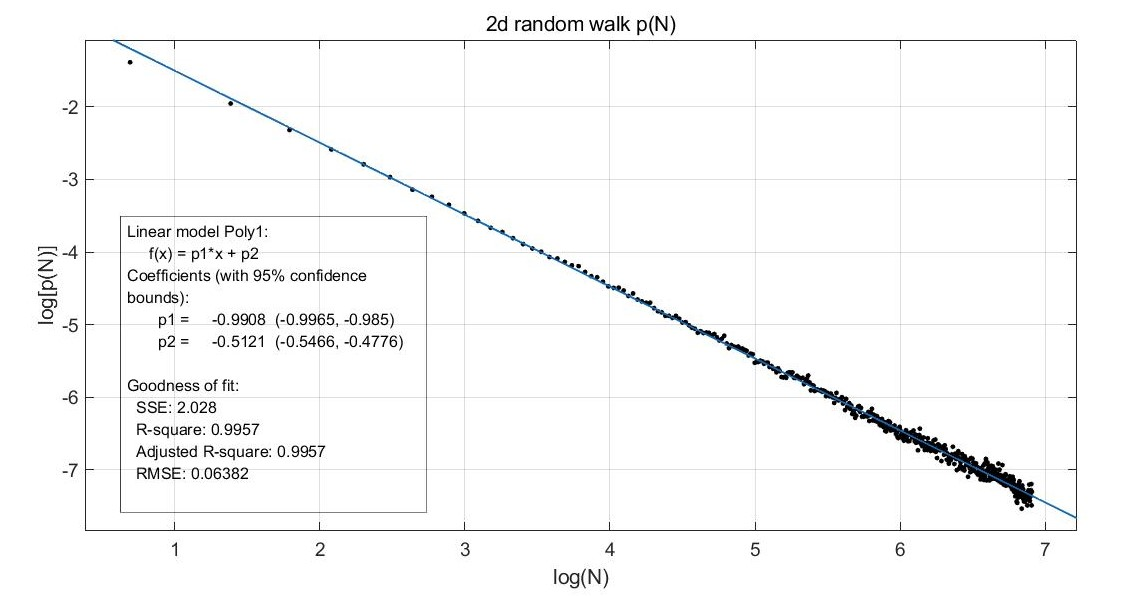
\includegraphics[width=6in]{../result_1/curve_2d.jpg}
		\caption{2d随机游走}
	\end{figure}
	
	
	\begin{flushleft}
		从拟合结果来看,一维的指数大约为$\nu=\textbf{-0.9908}$。这和理论近似的$\textbf{-1.0}$非常接近,且随着$N$的增大,吻合程度增大,这也符合对大$N$值近似展开的前提。
	\end{flushleft}
	
		\begin{figure}[H]
		\centering  %图片全局居中
		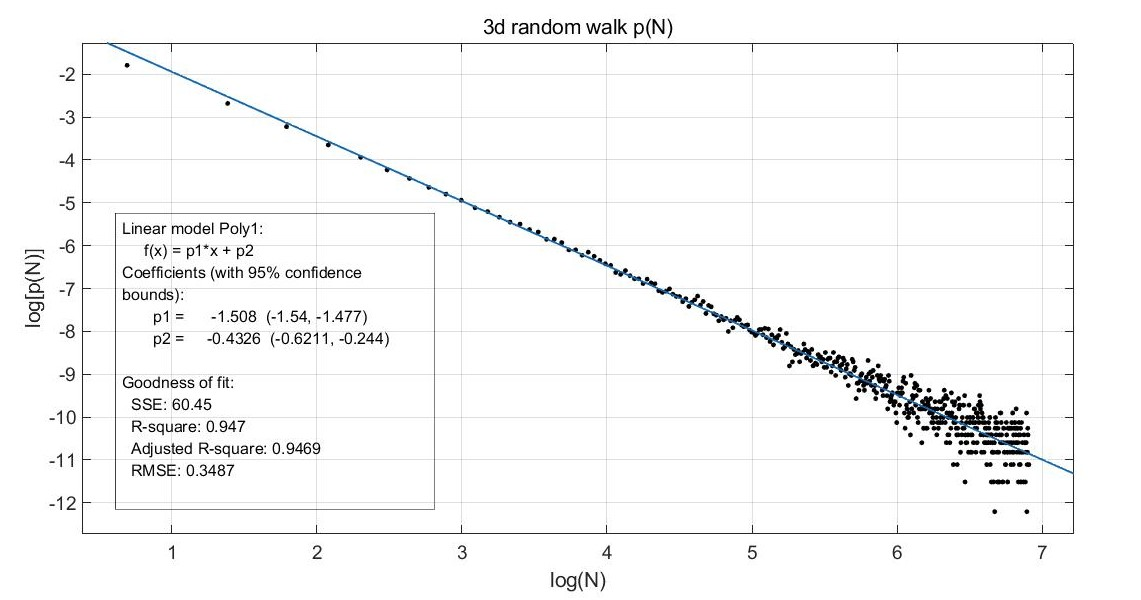
\includegraphics[width=6in]{../result_1/curve_3d.jpg}
		\caption{3d随机游走}
	\end{figure}
	
	\begin{flushleft}
		从拟合结果来看,一维的指数大约为$\nu=\textbf{-1.508}$。这和理论近似的$\textbf{-1.5}$非常接近,且一开始随着$N$的增大,吻合程度增大,这也符合对大$N$值近似展开的前提。并且由上面的理论推导可以指导,$p$确实也会略小于标度的$-1.5$次方关系,从而实际实验标度要略小于$-1.5$。但是需要注意的是,当$N$继续增大时,可能是由于笔者选取的系综数量还不够多,在大步长的时候会出现$log(p)$无穷大的点,因为没有粒子经过原点。另一个值得注意的是,由于系综取得不够大,在后面很大的$N$时出现的统计涨落会变大,体现在图上就是最后模糊的一片点集,这是由系综中系统数$M$不够大引起的,而非步长$N$的原因。
	\end{flushleft}
	
	\subsection{三维和二维的随机游走比较}
	
	做出系综中一个粒子的随机游走轨迹。
	在二,三维的轨迹如下:
	
		\begin{figure}[H]
			\centering  %图片全局居中
			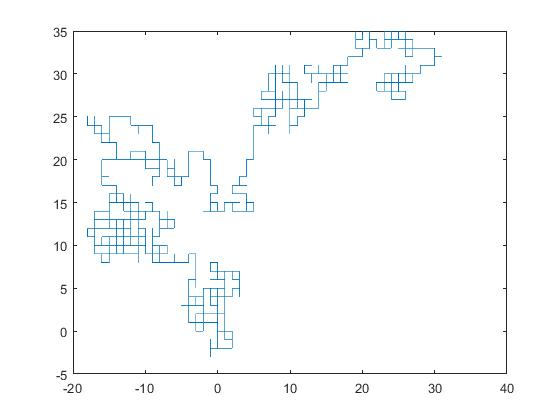
\includegraphics[width=6in]{../result_1/2d_xy}
			\caption{二维随机游走}
		\end{figure}
	
	\begin{figure}[H]
		\centering  %图片全局居中
		\subfigure[三维视图]{
			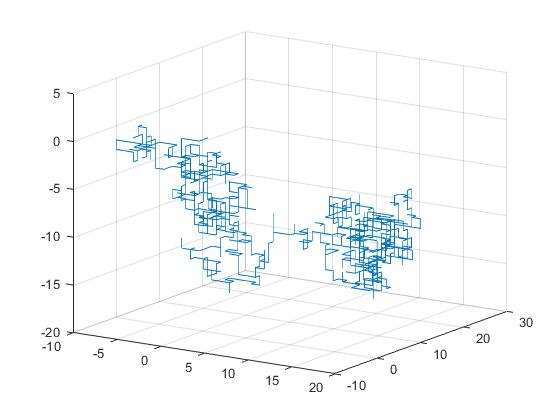
\includegraphics[width=0.45\textwidth]{../result_1/3d_xyz}}
		\subfigure[xy平面投影]{
			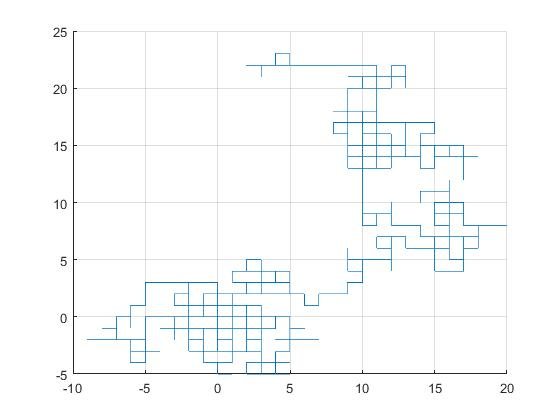
\includegraphics[width=0.45\textwidth]{../result_1/3d_xyz_xy}}
		\caption{三维随机游走}
	\end{figure}
	
	

%	\begin{figure}[H]
%		\centering  %图片全局居中
%		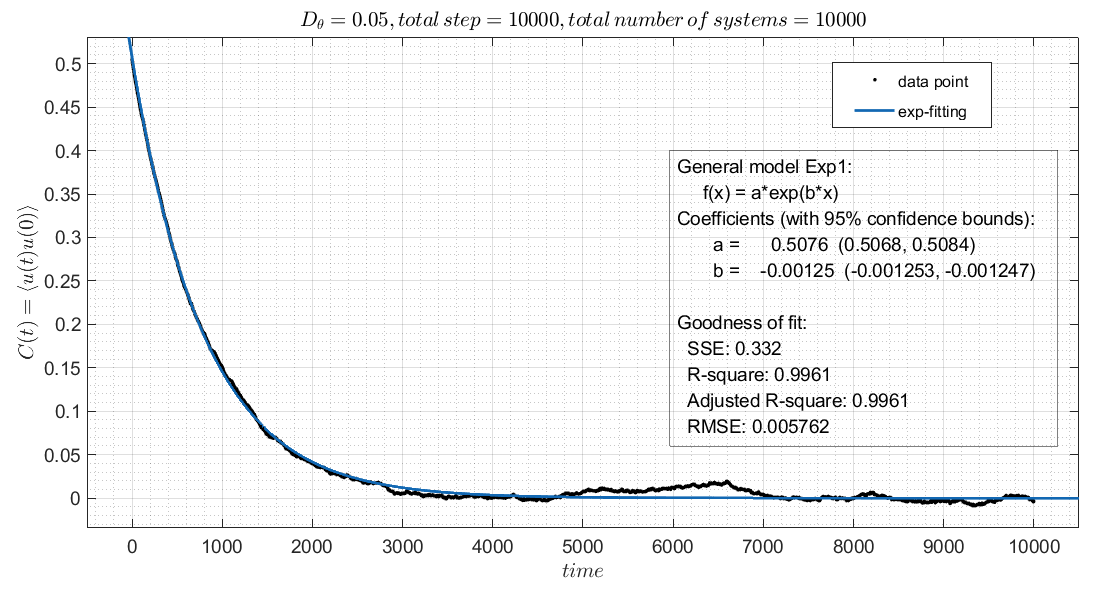
\includegraphics[width=6in]{rw}
%		\caption{拟合结果}
%	\end{figure}
%	
	\newpage

%\begin{figure}[H]
%	\centering  %图片全局居中
%	\subfigure[N=2]{
%		
%		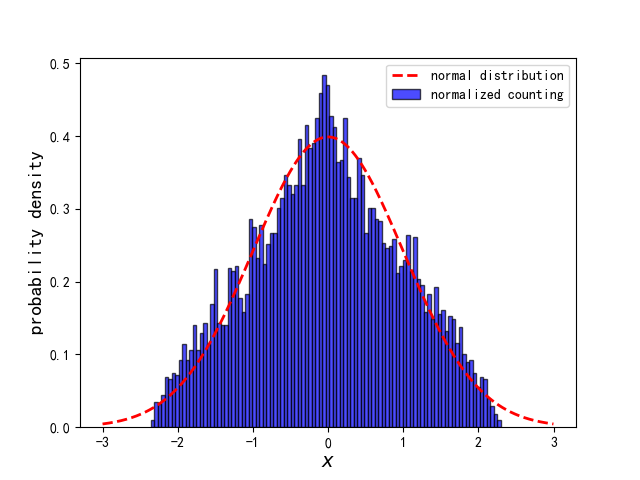
\includegraphics[width=0.45\textwidth]{../result/self_2.png}}
%	\subfigure[N=5]{
%		
%		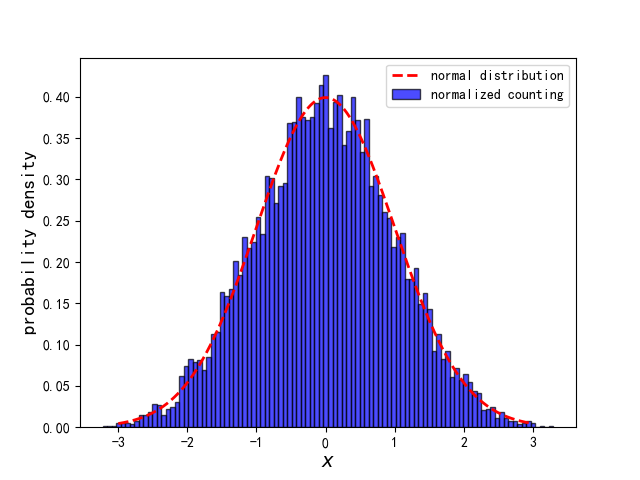
\includegraphics[width=0.45\textwidth]{../result/self_5.png}}
%	
%	\subfigure[N=10]{
%		
%		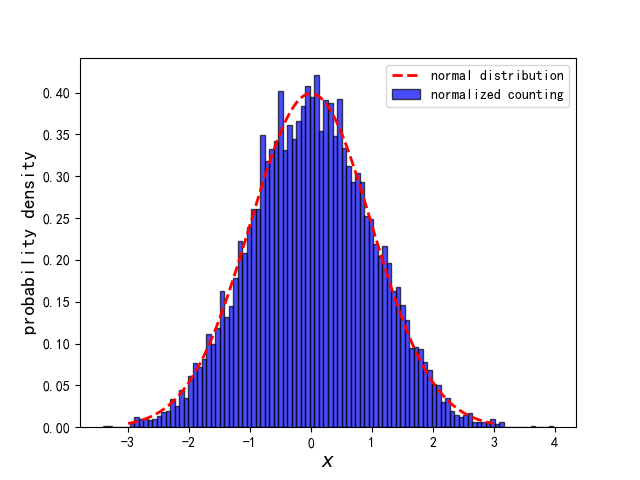
\includegraphics[width=0.45\textwidth]{../result/self_10.png}}
%	\subfigure[N=1000]{
%		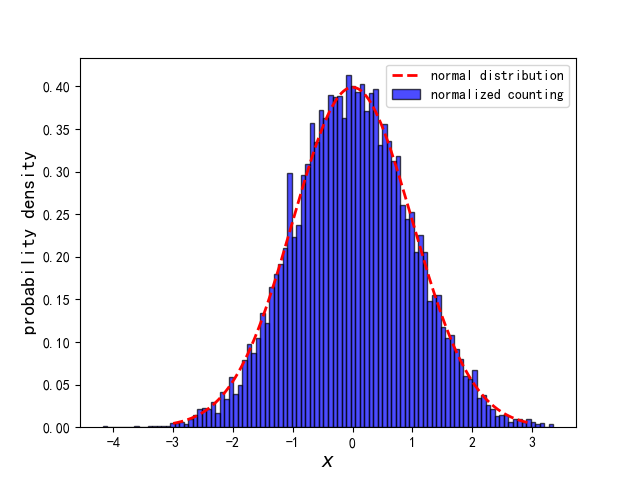
\includegraphics[width=0.45\textwidth]{../result/self_1000.png}}
%		
%	\caption{不同$N$下面的$Y$分布情况}
%\end{figure}


%		\begin{figure}[H]
%		\centering  %图片全局居中
%		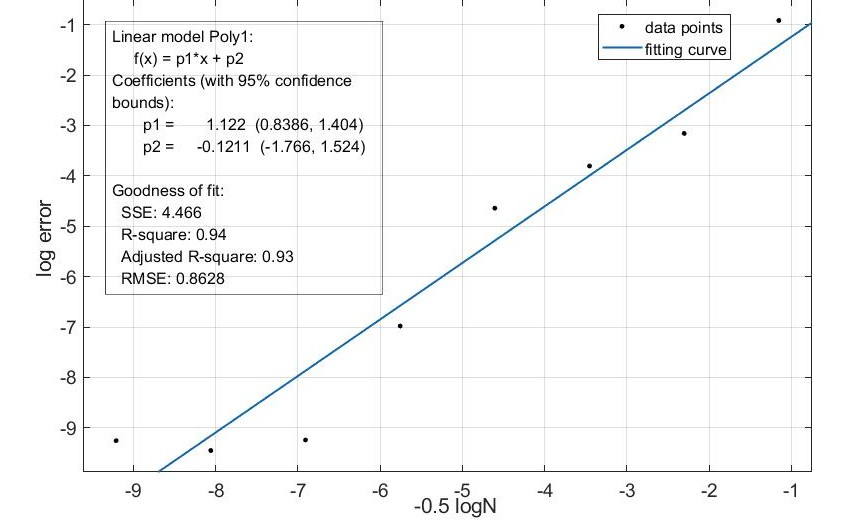
\includegraphics[width=6in]{../figure/single.jpg}
%		\caption{$log(\epsilon)-log(\frac{1}{\sqrt{N}})$}
%	\end{figure}
	

%	\begin{figure}[H]
%		\centering  %图片全局居中
%		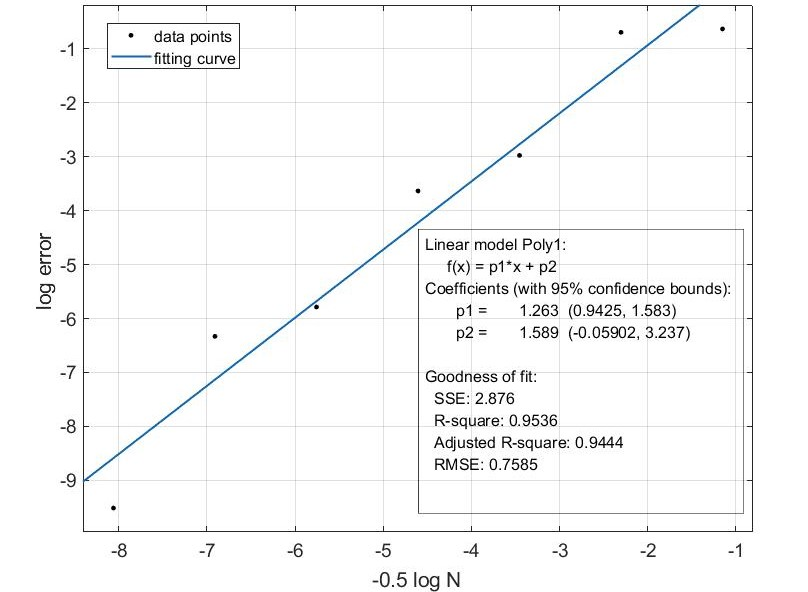
\includegraphics[width=6in]{../figure/multi.jpg}
%		\caption{$log(\epsilon)-log(\frac{1}{\sqrt{N}})$}
%	\end{figure}

	\newpage
	\section{总结}
	\begin{itemize}
		\item 本实验数值摸拟了$d=1,2,3$维随机游走的标度律,得到了和理论自洽的结果。
		\item 程序还需改进。有的地方动态分配多个大数组,明显减慢了运行速度。并且为了换不同的时间种子,用了几处$sleep$函数,也降低了运行速度。
	\end{itemize}
	
	
	\begin{thebibliography}{99}  
		\bibitem{ref1}
		Woess, Wolfgang. Random walks on infinite graphs and groups. Vol. 138. Cambridge university press, 2000.
	\end{thebibliography}
\end{document}